\chapter[Solution]{Solution}
\label{ch:solution}
This chapter is devoted to the implementation of the web application, which is the result of the bachelor thesis. It was realised according to the concept introduced in the previous chapter \ref{ch:concept} \nameref{ch:concept} to meet the stated requirements.

This application uses full-stack web framework as soon as it supports front-end interface, back-end services and databases development. The application uses client-server model, where front-end corresponds to the client side, and front-end is considered as server side. The following sections describe implementation of every technologies stack component.

    \section{Front-end}
    This section is devoted to the implementation of application, which runs on client side and provides interaction with him.
    
        \subsection{Angular framework}
        Front-end uses Angular, a platform and framework for building dynamic applications on the client side. Its primary programming language is TypeScript. Like any Angular application, the result application depends on features and functionality provided by libraries that are available as npm packages, and npm package manager was used to download and install them \cite[Node.js]{angular_getting_started}.
        
            \subsubsection{Angular modules}
            Angular provides modules, which provide components implementing common interaction patterns according to the Material Design specification \cite[Components]{angular_components}. Components such as Toolbar, Table, Paginator, Dialog, Expansion Panel etc. were used for creating fast, modern and consistent user interface.
    
            \subsubsection{Angular Reactive Forms module}
            Angular Reactive Forms module was used to create complex dynamic and nested forms. They allow storing inputs from the user or generate multiple nested forms with the same structure. They were used to create and edit courses, lessons and exercises, and also to solve the latter. As a result, it is possible to change the form view as soon as different exercise type is selected. Also they are used to add, remove and rename files at the code editors on exercise creation.
            
            Accuracy and completeness of the input is improved with the form validation, provided by the Form Group. The required fields change dynamically with the form itself.
    
        \subsection{External modules}
        Except Angular modules, application uses two external modules, which provide editors. Functionality and use of them is described in the following sections.
        
            \subsubsection{Quill module}
            The first one is based on Quill rich text editor. It was chosen because its component provides useful text formatting features, e.g. source code, quotations and headers. There is a view of a used quill editor at screenshot \ref{fig:quill}. This component is used to create and edit exercises description.
            
            The code editor is configured to store user input as HTML-string. The editor uses Angular DomSamitizer to sanitise these values, so it also meets a requirement of security.
    
            \begin{figure}[h]
                \centerline{
                    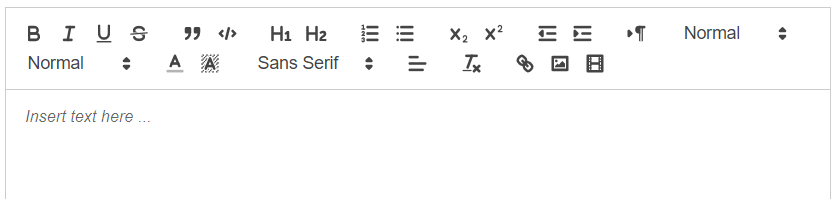
\includegraphics[
                    width=0.9\textwidth, width=\linewidth, frame
                    ]{images/quill.png}}
                \caption{Quill rich text editor component}
                \label{fig:quill}
            \end{figure}
            
            \subsubsection{Monaco module}
            The second module is based on Monaco code editor, which powers a high productivity Visual Studio Code editor. Its component was chosen because it has numerous tools to create a powerful development environment. The editor enables highlighting of the Java code, searching, suggestions, minimap, so the requirement of providing a close to conventional IDE was met. There is an example of use of Monaco editor module at screenshot \ref{fig:monaco}.
            
            \begin{figure}[h]
                \centerline{
                    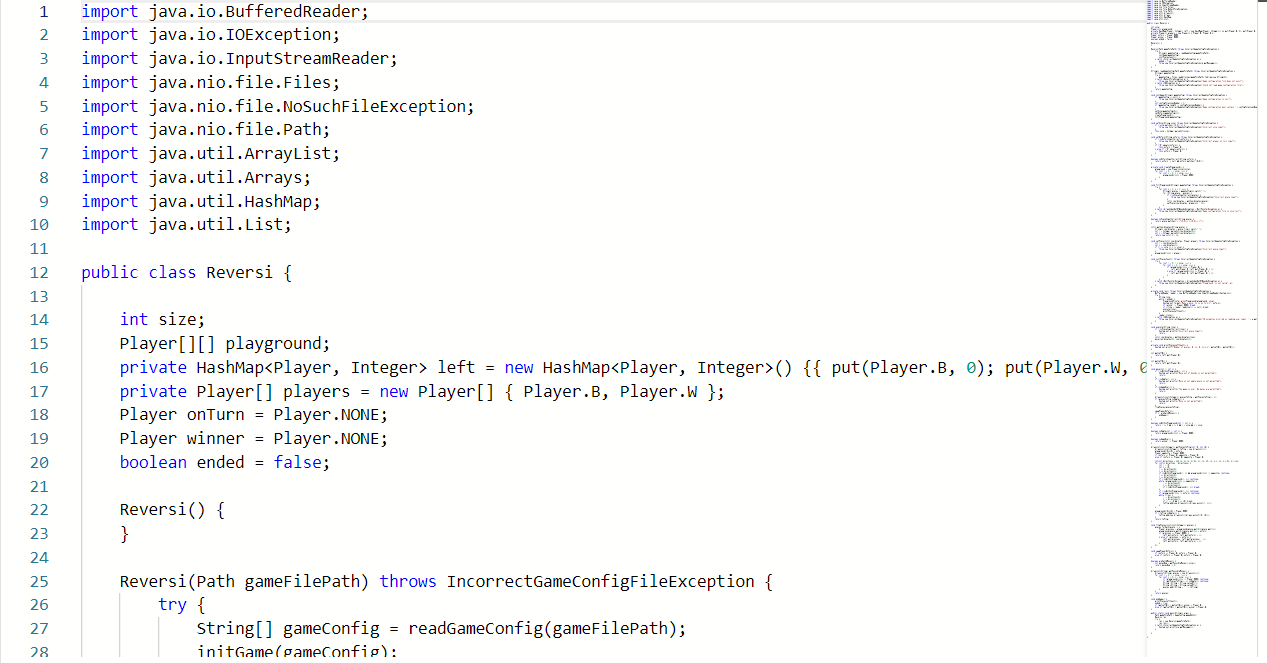
\includegraphics[
                    width=0.9\textwidth, width=\linewidth, frame
                    ]{images/monaco.png}}
                \caption{Monaco code editor}
                \label{fig:monaco}
            \end{figure}
    
    
        \subsection{Custom modules}
        Angular provides tools for making program modular. There are three modules in the application: courses, lessons and exercises. They contain components, routing modules, service providers. Components of these modules present data and define the view together with HTML templates. Routing modules enable navigation from one view to the next as users perform application tasks. The services are used for encapsulation of data access. The service providers handle sending requests to the server and retrieving the responses with use of HttpClient \cite[Architecture]{angular_getting_started}. The modules, components, routes and services were generated with use of Angular CLI, a command line interface.
    
        They are used to display pages or sections. Components are reusable, so some of them are used for different purposes, e.g. to create and edit a course, to manage a course and a lesson. Also they are used to display repetitive sections to avoid duplicates, e.g. show three same code editors with different content.
    
            \subsubsection{App module}
            App module is not quite custom as soon as it is the root module and every Angular application must have it. This module defines features, used by the whole application, e.g. the main navigation toolbar. This module imports Courses module and Not Found Module, described in the following sections.
    
            \subsubsection{Courses module}
            This module contains components for viewing and management the courses. It contains four components. Two of them, Manage and Upsert, are shared with imported Lessons and Exercise modules. The rest two components deal with courses only.
            
            Courses module contains course model to hold data and service providers to send and receive them from the server.
            
                \paragraph{Courses list component}
                This module is defined in App Module as a start page of the application. This component displays a list of courses, with general information. The table view was implemented with use of Angular Table module. Angular Paginator module provided component for pagination to limit the shown items number.
                
                There is an option of management the courses, which leads to Manage component.
                
                Example is shown on screenshot \ref{fig:courses}.
        
                \begin{figure}[h]
                    \centerline{
                        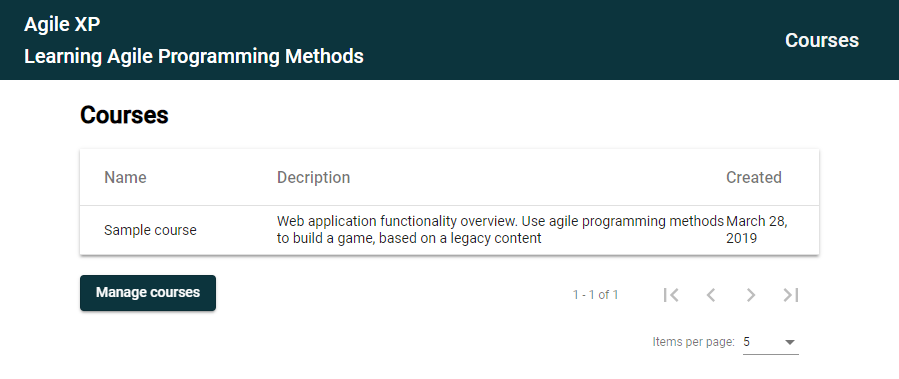
\includegraphics[
                        width=0.9\textwidth, width=\linewidth, frame
                        ]{images/courses.png}}
                    \caption{Courses list}
                    \label{fig:courses}
                \end{figure}
                
                \paragraph{Course detail component}
                This component provides detailed information about one of the courses, chosen from from the courses list. It provides a complete overview to acquaint with the course. There is an extension panel, implemented with use of Angular Extension Panel module, under the general information on the course, to list the course lessons, and to list the exercises from the lesson on click.
                
                Course detail component lead to Manage component to manage both lessons and exercises.
                
                Example is shown on screenshot \ref{fig:course-detail}.
                
                \begin{figure}[h]
                    \centerline{
                        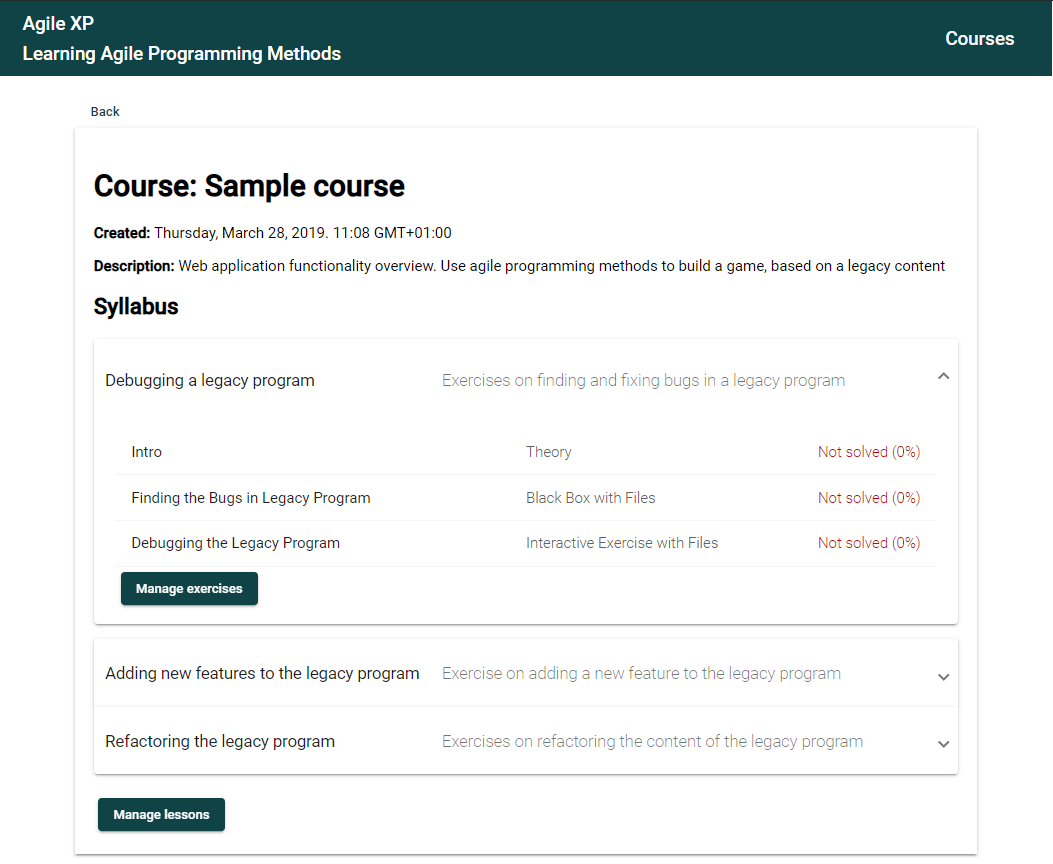
\includegraphics[
                        width=0.9\textwidth, width=\linewidth, frame
                        ]{images/course-detail.png}}
                    \caption{Course detail}
                    \label{fig:course-detail}
                \end{figure}
                
                \paragraph{Manage component}
                The previous components references to this module, as it was defined in the router of the Course module. This component provides tools for creating, editing, deleting, reordering the courses, lessons and exercises. The reason of this merge is that management has the same structure and mostly the same functionality for three manageable items.
                
                The Manage component contains abstract class to define general functionality, like creating, editing and deleting. Three classes for managing courses, lessons and exercises, inherit from it and use a common HTML template and styles. Lessons and exercises management is extended with reordering feature, implemented with use of Angular Drag and Drop module.
                
                Both create and edit buttons lead to Updert module, which is also used for different purposes.
                
                Example is shown on screenshot \ref{fig:manageExercises}.
                
                \begin{figure}[h]
                    \centerline{
                        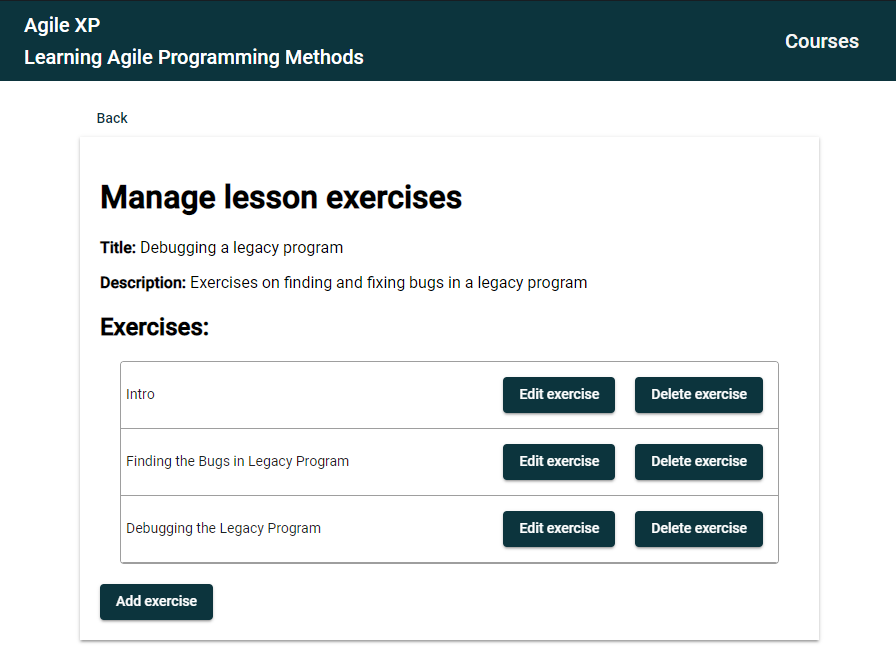
\includegraphics[
                        width=0.9\textwidth, width=\linewidth, frame
                        ]{images/manageExercises.png}}
                    \caption{Manage component}
                    \label{fig:manageExercises}
                \end{figure}
                
                \paragraph{Upsert component}
                The name of this module is a reference to a database management feature, which means a combination of \textit{insert} and \textit{update} \cite[ON CONFLICT Clause]{postgre_insert}. Upsert module is used to creation and editing the courses and lessons.
                
                The reason is the same as for Manage module. Exercises creation and editing is not that simple, to it required another module.
    
    
            \subsubsection{Lessons module}
            This module is imported by Courses module, so Lessons module can use its components. Lessons module also contains lesson model and services, and Courses module can access them. This module does not contain any component, and only uses shared components from the Courses module.
        
            \subsubsection{Exercises module}
            Exercises module is the most complex. It contains several models and services, and various components for one or many purposes.
        
                \paragraph{Exercise Upsert component}
                Exercise creating and editing is implemented with the same component, which contains various nested components. Angular Reactive Forms were used to create a dynamic form to interact with the user and store his input.  Content of fields, text and code editors from the nested components are bound to the form control and is processed on submit. This component also uses abstract component, inherited by creating and editing component.
                
                Non-dynamic part contains fields for exercise title, description and exercise type selector. Angular Form Field component was used for title, Quill rich text editor component was used for filling the description, and Angular Select was used for selecting an exercise type. This part is implemented with Create Intro component.
                
                When an exercise type is chosen, the form changes and the corresponding editors appear. The same component was used to place multiple editors with the same structure. The used form enables changing exercise type without losing data, and they would be available in the appeared editors.
                
                Each editor is implemented with Editor component. This uses tab view to represent several files. Content of any file may be manipulated with use of Monaco code editor. Angular Tab Module was used to create tabs, and buttons for renaming and deletion were added to them. The last tab contains button for adding new file. The default file name is ``filename.java``, and it may be changed in dialogue window, shown on screenshot \ref{fig:dialog}. The .java extension is added to a new file name from the input. Dialog component implemented the dialog with use of Angular Dialog module.
                
                \begin{figure}[h]
                    \centerline{
                        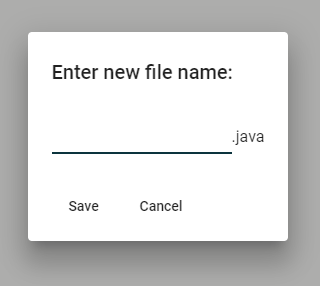
\includegraphics[
                        width=0.4\textwidth, frame
                        ]{images/dialog.png}}
                    \caption{Filename change dialog}
                    \label{fig:dialog}
                \end{figure}
                
                View of the whole component is shown on screenshot \ref{fig:editor-create}.
                
                \begin{figure}[h]
                    \centerline{
                        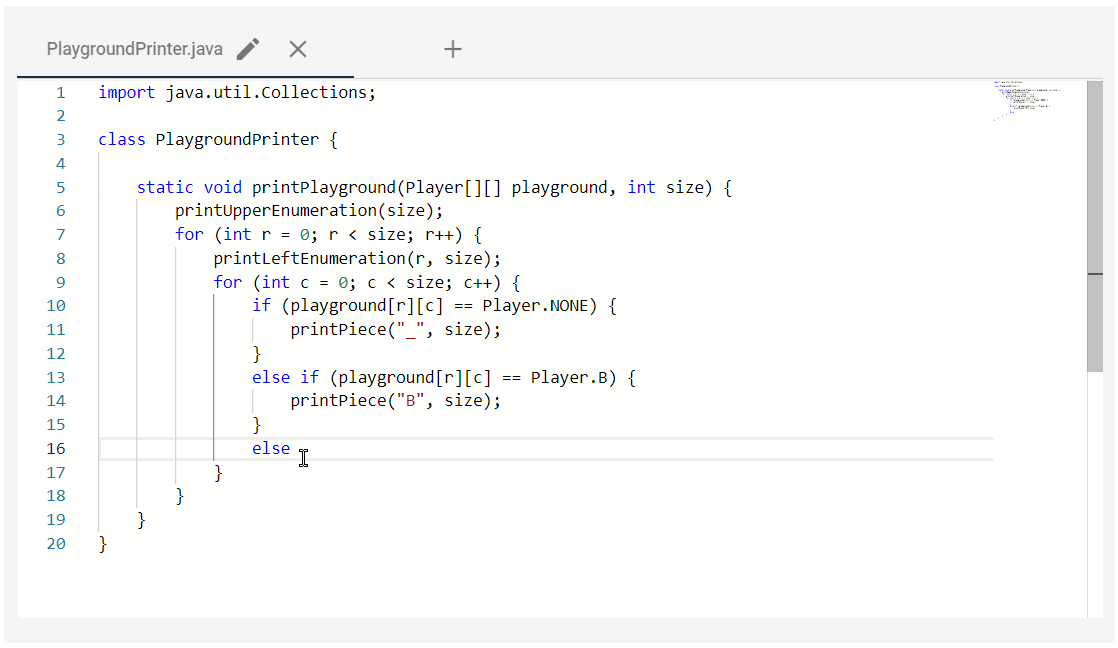
\includegraphics[
                        width=0.9\textwidth, width=\linewidth, frame
                        ]{images/editor-create.png}}
                    \caption{Editor element on exercise create or editing}
                    \label{fig:editor-create}
                \end{figure}
                
                The dynamics of the form was used to fulfil a required feature of convenient creation of two versions of source code, tests and text files. Upsert Editors component implements this feature. On exercise creation or update, there is an editor for a hidden version, and there is a select component below. The component contains two options for the shown version. The first option, ``the same``, is used when an exercise author wants the shown version to be the same a hidden. As a result, the content of the editor would be saved as both hidden and shown version. And the second option, ``custom``, is used to create or edit a different shown version, and an new editor element appears. Some of the exercise types require only a hidden or shown version of source code or test, so there is no select component.
                
                Create Submit component displays a submit button, which is enabled as soon as the form input is valid. On submit, there would appear a notification telling if the data were saved successfully. When cheating new exercise, there would be an suggestion to create another one.
                
                Submitting of the exercise is realised with Exercise Creator and Editor services, called from the Submit Component. Both of them inherit from abstract Exercise Saver service.
    
                \paragraph{Exercise Solve component}
                This component has a complex structure too, but this component is used only for solving the exercises. Interaction with the user and storing his input was also implemented with use of dynamic forms.
                
                When solving an exercise, its view is determined by its type. Every exercise type has view and functionality according to the concept, described in a section \ref{subsec:exercise-types} \nameref{subsec:exercise-types}. Exercise Solve component determines the number, content of the editors and a nested form, to which an editor is bounded to.
                
                Solve Editor component consists of an editor, which uses code editor component from Monaco module, and a version control section. Version control enables resetting the editor content and loading content from a submitted version. When an exercise is chosen, a dialog appears. It views eight most recent submitted solutions. User may require getting more from the server with ``Load more button``, and use paginator to display them. A typical code editor is illustrated on screenshot \ref{fig:editor-solve}.
                
                + image for version control
                
                \begin{figure}[h]
                    \centerline{
                        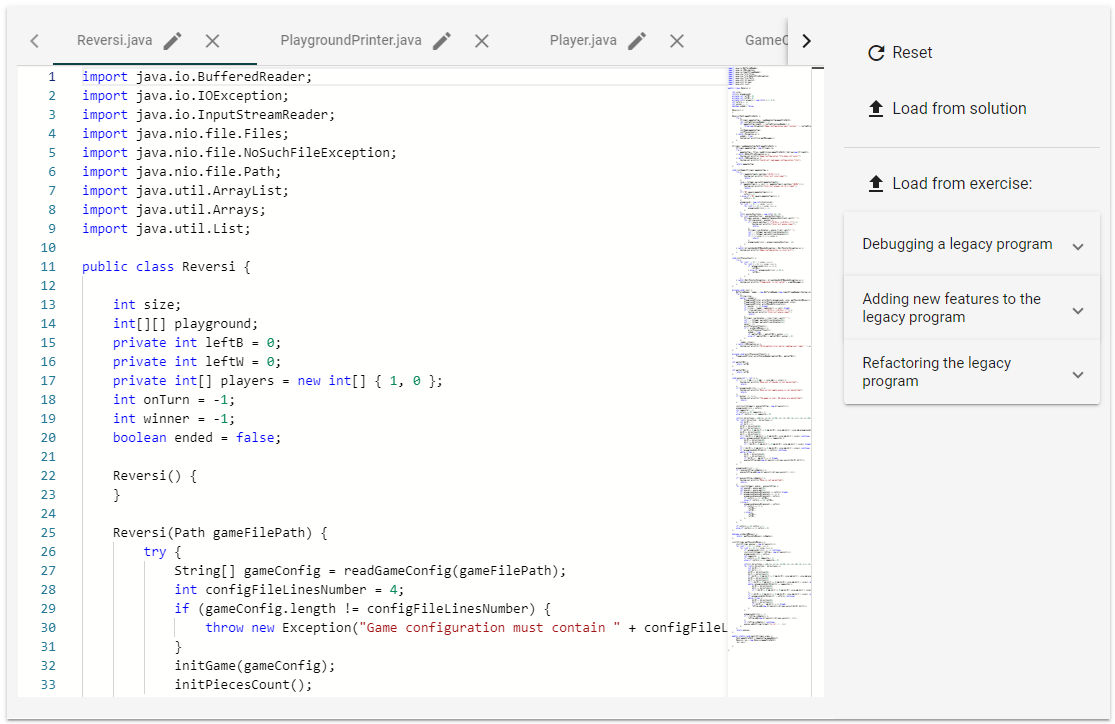
\includegraphics[
                        width=0.9\textwidth, width=\linewidth, frame
                        ]{images/editor-solve.png}}
                    \caption{Editor element}
                    \label{fig:editor-solve}
                \end{figure}
                
                Every exercise contains a Intro component for displaying a description of the exercise. The description content was created with use of rich text editor component of Qill module, and its content is formatted. There is an example at screenshot of the exercise description \ref{fig:description}.
                
                \begin{figure}[h]
                    \centerline{
                        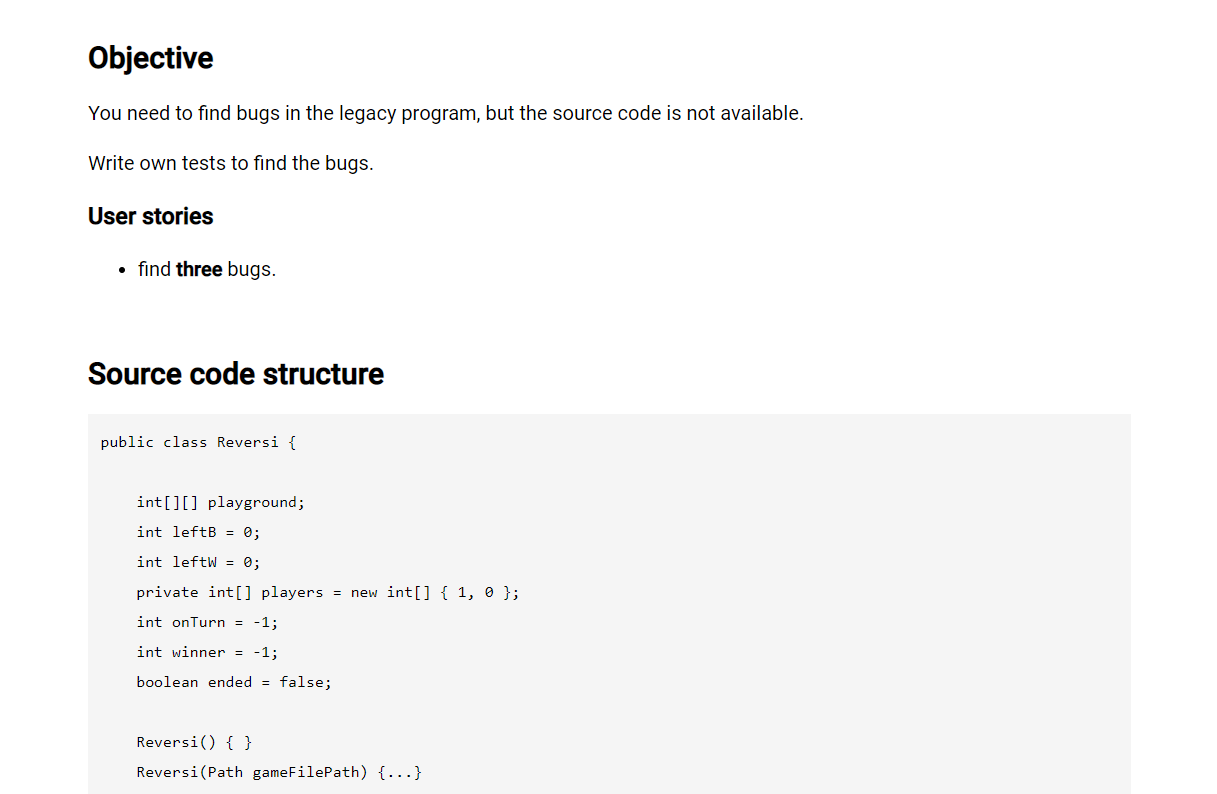
\includegraphics[
                        width=0.9\textwidth, width=\linewidth, frame
                        ]{images/description.png}}
                    \caption{Exercises description}
                    \label{fig:description}
                \end{figure}
                
                The pages for solving the exercises contain two equal toolbars, one on the top and second on the bottom of the page. They are implemented with Toolbar component with use of Angular Toolbar. Route module defines navigation back to Course Detail component with button, or navigation to previous or next exercise. Also there is a flag representing the progress on the solving current exercise. An example of the toolbar view is available at screenshot \ref{fig:toolbar}. They change dynamically on an exercise change and restrict from navigating to not available exercise.
                
                \begin{figure}[h]
                    \centerline{
                        
\includegraphics[
                        width=0.9\textwidth, width=\linewidth, frame
                        ]{images/toolbar.png}}
                    \caption{Exercises toolbar}
                    \label{fig:toolbar}
                \end{figure}
                
                Solve Run component is responsible for running the estimation of the submitted result. Firstly, when ``Run`` button is clicked, an output area appears and it contains ``Loading...`` message. Submitted source code, tests, files, solution itself and estimation should be saved to database, and they references, so they should be sent to the server in order. Sending requests to the server runs asynchronously with use async-await feature to make code more readable and call functions sequentially without making code hell of nested calls and conditions. The received estimation is shown to the user in the output area.
    
            \subsubsection{Not found module}
            This module is imported by the App Module, and is used for redirection to it if the routing modules does not contain a requested path.
    
    
    \section{Back-end}
    This section describes implementation of application, which runs on server and is responsible for handling business logic and data storage.
    
    The server side Java application uses Spring Framework, and is managed with Maven. HTTP requests are handled by Controller components. Service components are used to implement business logic on a separate layer. One of them, Estimator Service component, receives estimation from estimation module, which creates it with Estimator-Java Component. Every data entity has own Repository component, which extends CrudRepository to provide CRUD functionality for the entity class that is being managed.
    
        \subsection{Virtual Sandbox}
        Virtual Sandbox is used to fulfil a security requirement, stated in \ref{subsec:security} \nameref{subsec:security}. The result application runs potentially harmful running of the code, provided by user, in a docker container. Compilation may be performed on server, and application would be still secure. But it would require dependencies, which may not be available on server. This section describes virtual sandbox usage.
        
        When server gets a request to estimate the solution, it gets an object with Request Body annotation, which is mapped to a domain object. It is deserialised to a Java object, which contains objects describing the solution files. They are stored to a named by solution is temporary file, stored at an uploading directory. Storage package contains tools for managing files in this uploading directory.
        
        Then Dockerfile with archived Java program are copied to the temporary solution folder. The next step is running the container. Docker Client plugin, provided by Spotify, contains tools for working with Docker. A class was created to use them, it takes care of building an image, container creation, starting it, getting an estimation file content and destroying the container. The result is parsed from JSON format, and based on it estimation object it created.
        
        
        \subsection{Estimating module}
        Estimating module is realised as Java program, which runs in Docker container. It uses Spring framework and Maven as well as a server application.
        
        Server application stores Dockerfile and jar of the program. On beginning of the estimation process, these files are moved to a temporary directory for solution. 
        
        Instead of executing commands from the server application or defining them in Dockerfile, the estimator program runs in the Docker container. It brings such a benefit as modularity, because it becomes easier to add more supported for estimation programming languages. 
        for writing the  the server application may use this or another such a module, depending on the program. Also it brings an opportunity to define the output of compilation, testing, error messages.
        
        The estimator program contains two classes for estimating a solution. The first class is responsible for exercise type \textit{Interactive exercise} and \textit{Interactive exercise with Files}, and the second handles \textit{Black Box} with \textit{Black Box with Files}. The both classes extend abstract class Estimator and implement estimation function, which starts the process.
        
        The result of the estimation is hold in an instance of Estimation class. It has an attribute \texttt{value}, which represents the progress percentage. For \textit{Interactive exercise (with Files)} type, the progress means how much tests were passed out of their total amount. Result class of JUnit API collects and summarises information from running multiple tests, but it does not provide information on total tests number. However, this number can be received during the tests running with JUnit API. TestResult class was created to store the total tests number, it extends Result class and adds a necessary attribute. Finally, the test result with compilation results are stored in an instance of Estimation class.
        
        The estimation result is created with converting the estimation object into JSON string with use of Gson plugin from Google. This output is written to a text file. Docker Client plugin enables getting an archive of a filesystem resource in a container, so the file with estimation can be read with the server application.
        
        Another way to deliver the result to the server is printing it to the console, and Docker Client may receive it. This simple solution has one problem. When solution program prints to console, its output also would be received by the server. As a result, writing the result to the file is more efficient.
    
    
    \section{Database}
    The resulting web application uses PostgreSQL relational database management system. The entity-relationship model of the database system should have been transformed into relation model for database creation and further implementation.
    
    Most of the entities are in many-to-one, one-to-many or one-to-one relationship. These relationships were transformed with use of references and unique constraints.
    
    The set of entities \texttt{exercise content} has the same attributes as the entities, which are in a subset relationship with it. Single Table strategy was used for transformation. As a result, all the subsets are stored in the same table \texttt{exercise content}, and are distinguished by \texttt{exercise content type} attribute. Hibernate Inheritance Mapping was used to implement this relation as inheritance, a Single Table inheritance strategy was used. The same approach was used on transformation from entity-relationship model to relation model for table \texttt{solution content} and subsets of its entities.
    
    
\begin{center}
\begin{figure}
\begin{tikzpicture}

\umlclass{courses}{
    id \textit{serial}\\
    name \textit{text}\\
    description \textit{text}\\
	created \textit{timestamp}\\
}{}

\umlclass[above=1.5 of courses]{lessons}{
    id \textit{serial}\\
	name \textit{text}\\
    description \textit{text}\\
    index \textit{int}\\
    created \textit{timestamp}\\
	course\_id \textit{int}\\
}{}

\umlclass[above=1.5 of lessons]{exercise content}{
    id \textit{serial}\\
    filename \textit{text}\\
    content \textit{text}\\
    exercise\_content\_type \textit{text}\\
    exercise\_id \textit{int}\\
}{}

\umlclass[above=1.5 of exercise content]{solution content}{
    id \textit{serial}\\
    filename \textit{text}\\
    content \textit{text,}\\
    solution\_content\_type \textit{text}\\
    solution\_id \textit{int}\\
}{}

\umlclass[right=1.5 of solution content]{solutions}{
    id \textit{serial}\\
    created \textit{timestamp}\\
	exercise\_id \textit{int}\\
}{}

\umlclass[below=4 of solutions]{exercises}{
    id \textit{serial}\\
	name \textit{text}\\
    description \textit{text}\\
	index \textit{int}\\
    created \textit{timestamp}\\
	lesson\_id \textit{int}\\
    type\_id \textit{int}\\
}{}

\umlclass[right=1 of solutions]{solution estimation}{
    id \textit{serial}\\
	estimation \textit{text}\\
	value \textit{int}\\
    solved \textit{boolean}\\
    created \textit{timestamp}\\
	solution\_id \textit{int}\\
}{}

\umlclass[right=1.5 of exercises]{bugs number}{
    id \textit{serial}\\
    exercise\_id \textit{int}\\
    number \textit{int}\\
}{}

\umlclass[right=2 of courses]{exercise types}{
    id \textit{serial}\\
	name \textit{text}\\
	value \textit{text}\\
}{}

\umldep[anchors=330 and 175]{solution content}{solutions}
\umlHVHdep[arm1=0.4, anchors=333 and 35]{solutions}{exercises}
\umldep[anchors=218 and 13]{solution estimation}{solutions}
\umlHVHdep[arm1=-0.5, anchors=222 and 170]{lessons}{courses}
\umldep[anchors=220 and 25]{exercises}{lessons}
\umlHVHdep[arm1=0.5, anchors=310 and 5]{exercises}{exercise types}
\umldep[anchors=333 and 145]{exercise content}{exercises}
\umldep[anchors=172 and 35]{bugs number}{exercises}

\end{tikzpicture}
\caption{Relational model of system data}
\label{database}
\end{figure}
\end{center}

    
    
    
%%%%%%%%%%%%%%%%%%%%%%%%%%%%%%
% ERROR HANDLING
% To make the web application robust, errors handling should be done efficiently. Such an approach provides informative error messages and good user experience.

